\documentclass[10pt]{article}
\usepackage[a4paper]{geometry}
\usepackage{amsmath}
\usepackage{amssymb}
\usepackage{tocbibind}
\usepackage{graphicx}
\usepackage{hyperref}
\usepackage{mdframed}
\usepackage{subfiles}
\usepackage{titlesec}
\usepackage[dvipsnames]{xcolor}

%%%%%%%%%%%%%%%%%%%%%%%%%%%%%%%%%%%%%%%%%%%%%%%%%%%%%%%%%%%%%%%%%%%%%%%% Setups
\newcommand{\Eq}[1]{Equation~\ref{eq:#1}}
\newcommand{\Fig}[1]{Figure~\ref{fig:#1}}

\newenvironment{textbox}[1]
{%
  \mdfsetup{%
    frametitle={\colorbox{white}{\space#1\space}},
    frametitleaboveskip=-\ht\strutbox,
  }
  \begin{mdframed}
}
{
  \end{mdframed}
}

\setlength\parindent{0pt}
\setlength\parskip{1.2ex}

\graphicspath{{./fig/}}

\hypersetup{%
  hidelinks,
  colorlinks,
  citecolor={YellowOrange!85!black},
  linkcolor={Aquamarine!85!black},
  bookmarksopen=true,
  bookmarksnumbered=true,
  linktoc=all,
  pdfauthor=Jihang Li,
}

\title{Notes of ``Visual Relationship Detection with Language Priors''}
\author{Jihang Li}
%%%%%%%%%%%%%%%%%%%%%%%%%%%%%%%%%%%%%%%%%%%%%%%%%%%%%%%%%%%%%%%%%%%%%%%%%%%%%%%

\begin{document}
\maketitle
\tableofcontents

%%%%%%%%%%%%%%%%%%%%%%%%%%%%%%%%%%%%%%%%%%%%%%%%%%%%%%%%%%%%%%%%%%%%%% Abstract
\section*{Abstract}%
\label{sec:abstract}
A model is proposed to train visual models for objects and predicated
individually and later combines them together to predict multiple relationships
per images. Improvement is done by leveraging language priors from semantic
word embeddedings to finetune the likelihood of a predicted relationship.

%%%%%%%%%%%%%%%%%%%%%%%%%%%%%%%%%%%%%%%%%%%%%%%%%%%%%%%%%%%%%%%%%%%%% Chapter 5
\setcounter{section}{4}
\section{Experiments}%
\label{sec:experiments}
The evaluation metrics reported in this paper is \textbf{recall@100} and
\textbf{recall@50} (refer to
\href{http://calvin.inf.ed.ac.uk/wp-content/uploads/Publications/alexe12pami.pdf}
{Measuring the Objectness of Image Windows}). \textbf{Recall@x} computes the
fraction of times the correct relationship is predicted in the top $\mathbf{x}$
confident relationship predictions.

\begin{textbox}{\textit{Original Texts}}
Even if the prediction is correct, mAP would penalize the prediction if we do
not have that particular ground truth annotation.
\end{textbox}

\begin{figure}[htpb]
  \centering
  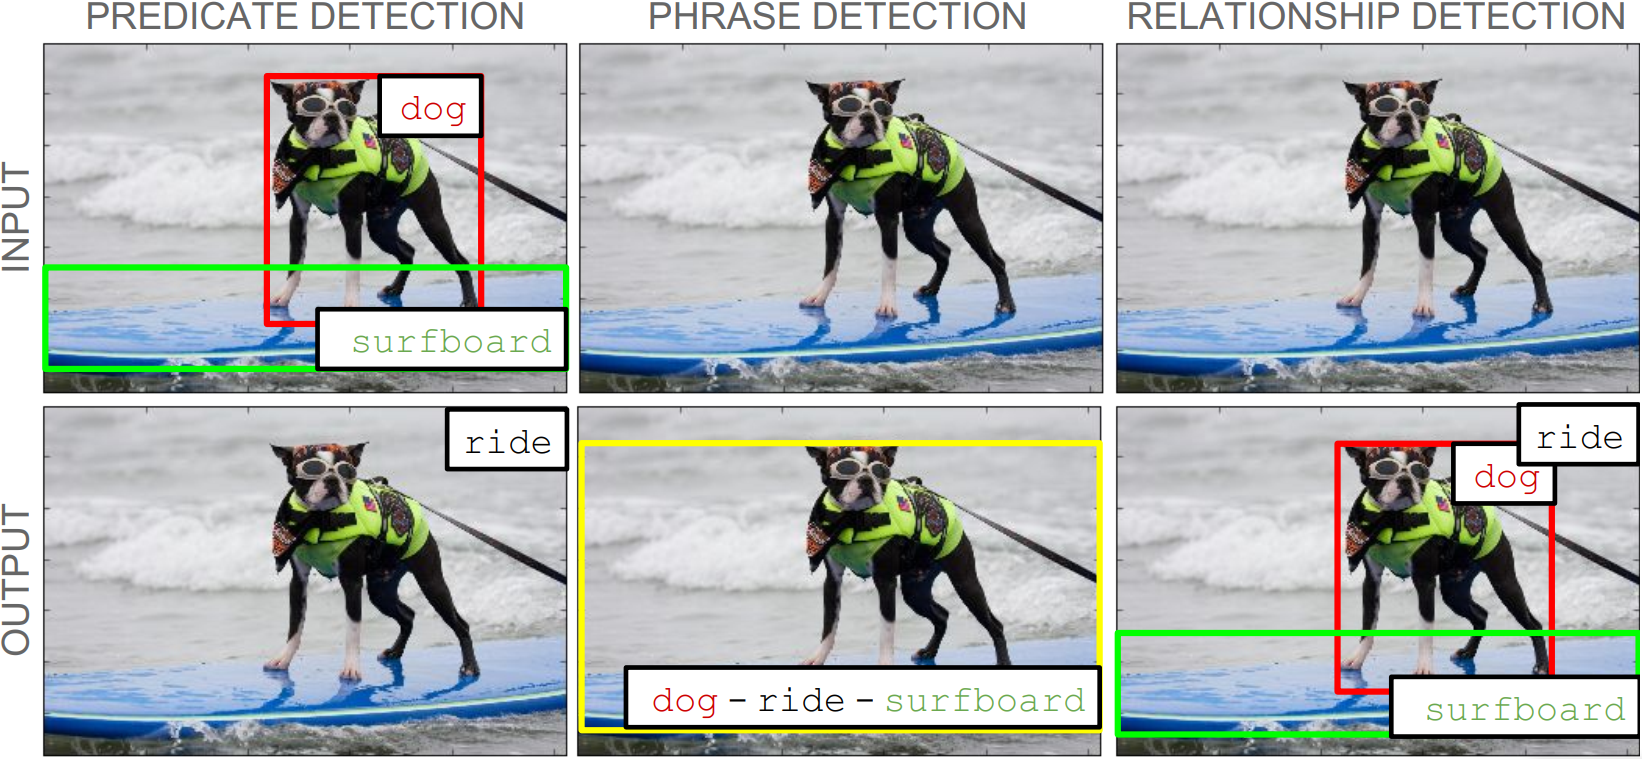
\includegraphics[width=0.8\linewidth]{fig_5.png}
  \caption{We evaluate visual relationship detection using three conditions:
    predicate detection (where we only predict the predicate given the object
    classes and boxes), phrase detection (where we label a region of an image
    with a relationship) and relationship detection (where we detect the
    objects and label the predicate between them).}%
  \label{fig:5}
\end{figure}

\end{document}
